\chapter{Dynamische Datenschemas in relationalen Datenbanken}

Um die Herausforderung, dynamische Datenschemas in Datenbanken abzuspeichern, besser zu verstehen, werden in diesem Kapitel die Grundlagen von relationalen Datenbanken näher betrachtet. Anschließend werden verschiedene Lösungswege in relationalen Datenbanken für die vorlegende Aufgabenstellung beschreiben.

%\section{Begriffe und Geschichte}
\section{Geschichte und Grundlagen}

Da die direkte Ablage von Programmdaten in Dateien zur langfristigen Speicherung sich schnell als sehr unflexibel herausstellte, wurde bereits 1963 das erste \ac{DBMS}, das IDS, von Bachman entwickelt\cite{Haigh.2016}. Obwohl damals die Hardware und die Speichermedien, hauptsächlich Tapes, die größeren Herausforderungen waren, besitzt \ac{IDS} viele Aspekte moderner \ac{DBMS}, unter anderem die Verwaltung von Metadaten über die gespeicherten Daten und die Möglichkeit, dass verschiedene Programme auf Basis der selben Datenbank arbeiten. Spätere Versionen beherrschten bereits die Verarbeitung von Online-Transaktionen. Daten in \ac{IDS} wurden in einer hierarchischen Struktur abgelegt.
Die heute dominierende Form von Datenbanken und deren relationales Modell wurden erst später von Ted Codd entwickelt\cite{Codd.1970}. Der Begriff Relation stammt aus der Mengenlehre und beschreibt eine Menge von n-Tupel, d.h. von Folgen mit einer festen Menge von Elementen.
Die einzelnen Skalare bzw. Werte an den Stellen eines Tupels können nur eine, für diese Stelle vorbestimmte, Form annehmen. Die jeweilige Stelle wird Attribut genannt und die möglichen Werte Wertebereich. Ein Tupel wird mit einem Primärschlüssel identifiziert. Mit diesem Schlüssel können Referenzen zwischen Tupeln in verschiedenen Relationen indiziert werden.
Das relationale Datenmodell wird basierend auf den Strukturen, die sich aus den mathematischen Grundlagen ergeben, meist mit Tabellen beschrieben. Eine Relation ist eine Tabelle, die Tupel werden zu Reihen und Attribute werden mit Spalten visualisiert.
Der erste Vertreter von relationalen Datenbanken, System R, verwendete die erste Implementation der \ac{DBMS}-Interaktionssprache \ac{SQL}\cite{Chamberlin.1981}. Modernes \ac{SQL} beinhaltet folgende Sprachen die zur Datenhaltung benötigt werden\cite{Mertens.2017}:

\begin{itemize}
\item \ac{DML}
enthält Befehle, mit denen Daten in der Datenbank modelliert, d.h. Einträge eingefügt und bearbeitet, werden können.

\item \ac{DDL}
wird verwendet, um eine konkrete Instanz des Datenmodels zu erstellen. Das entstehende Konstrukt heißt Datenschema.

\item \ac{DCL}
beinhaltet Befehle zur Anpassung von Rechten auf die Daten.
\end{itemize}

Die Kombination einer sehr flexiblen Sprache in SQL und einem Modell, das große Teile der benötigten Daten von Unternehmen hocheffizient abspeichern kann, ermöglichten den Aufstieg der relationale Datenbanken\footnote{Genau genommen handelt es sich um SQL Datenbanken. Die umgangssprachliche Verwendung der Bezeichnung \textit{relationale Datenbank} entspricht nicht der Definition des Begriffs. Ein Unterschied zwischen der Definition und der heutigen Implementationen ist z.B. die Möglichkeit, NULL Werte abzuspeichern. Das ist jedoch nicht Teil der Spezifikation der relationalen Datenbank.} zu ihrer heutigen Dominanz auf dem Markt. Trotzdem besitzt dieses Modell mehrere Schwächen.

Eine Schwäche ist die mangelnde Dynamik des Datenschemas, welche diese Arbeit motiviert. Änderungen am Schemas sind grundsätzlich möglich, sind jedoch nicht sehr performant. Die ANSI-SPARC Architektur für Datenbankschemas verspricht logische Datenunabhängigkeit. In der Praxis sind jedoch meist externe Anwendungen und das Schema direkt gekoppelt. Für Softwareprojekte werden bei Datenbankänderungen oft Migrations-Scripts angelegt, die das Datenbankschema in einem großem Schritt umwandelt. Volatile und dynamische Datenstrukturen können nur mit Umwegen, die im Anschluss betrachtet werden, abgespeichert werden.
Eine andere Schwäche ist die Skalierbarkeit der Datenbanken, verglichen mit speziell entwickelten verteilten Datenbanken\cite{Pokorny.2013}. Fehlende Partitionierungsmethoden erschweren die horizontale Skalierung und erfordern stattdessen stärkere Hardware um größere Datenmengen abzulegen und mehr Transaktionen zu verarbeiten.  


\section{Datenbank Normalisierung: Normalformen}



Datenbanknormalisierung ist ein Vorgang während der Definition des Datenmodels zur Minimierung von Datenanomalien und Eliminierung von Redundanz. Mithilfe der Normalformen werden Strukturen definiert, die die Abhängigkeiten zwischen den Daten einschränkt. Die Normalisierung ist ein Vorgang mit Vor- und Nachteilen.

\begin{itemize}
\item \textbf{Datenanomalien} \\
Es existieren verschiedene Arten von Datenanomalien. Update-Anomalien entstehen, wenn die Bearbeitung von Daten zu inkonsistenten Zuständen durch Duplikate führen kann. Einfüge-Anomalien beschreiben den Zustand, wenn neue Entities nicht ohne zusätzliche Attribute in die Datenbank eingefügt werden können. Lösch-Anomalien treten durch Datenverluste auf. Diese Anomalien lassen sich auf duplizierte und schlecht strukturierte Datenmodelle zurückführen, die durch die Normalisierung verhindert werden.
\item \textbf{Speicherverbrauch} \\
Ein Nebeneffekt der Eliminierung von Duplikaten in der Datenbank ist die Verringerung des Speicherbedarfs der Datenbank.
\item \textbf{Performanz} \\
Die Normalisierung teilt Informationen, die zunächst in einer einzigen Tabelle gespeichert waren, oft in mehrere Tabellen auf, je nach den Abhängigkeiten der Daten. Um diese Verhältnisse in einer Abfrage wieder darzustellen und abzulaufen müssen unperformante join Operationen durchgeführt werden. Dadurch steigt die durchschnittlichen Antwortzeit.
\end{itemize}

Es existieren mehrere Normalformen, die jeweils die Struktur des Modells immer weiter einschränken. Ein nicht-normalisiertes Modell wird auch nullte Normalform genannt.
%erste normalform -> erzeugung atomarer werte, eliminierung von tupel
Die erste Normalform bringt die Einschränkung, das alle Attribute nur einfache Werte annehmen dürfen. Das bedeutet, dass ein Wert keine Menge sein darf und keine innere Struktur, die weiter verarbeitet werden muss, beinhalten darf. Diese Eigenschaft wird auch als atomar bezeichnet.
%Die zweite Normalform besagt, dass jedes nicht-Schlüssel Attribut voll vom Schlüsselattribut abhängen muss und sich die Daten bereits in der ersten Normalform befinden müssen.
Die bekannteste und häufig angestrebte Normalform ist die dritte nach Boyce/Codd Normalform. 

\begin{quote}
"`3. Normalform (Boyce/Codd): Eine Relation R in l.NF ist auch in 3.NF, wenn jede Determinante in R ein Schlüsselkandidat ist. (Determinante heißt ein Attribut oder eine Attributskombination, von  welchem irgend ein anderes Attribut von R voll abhängig ist.)"' \cite[Seite 52]{Zehnder.1985}
\end{quote}




Zusätzlich existieren höhere Normalformen, die die Strukturen weiter eingrenzen.

Höhere Normalformen sind in praktischen Umgebungen seltener in Gebrauch, da bereits die dritte Normalform alle Redundanzen entfernt. \cite{Zehnder.1985}






%realtionales Modell
%realation -> set of tupels
%tupel -> ordered set of attribut values(name+type)
%verweise zwischen relationen per einzigartiger schlüssel, meißt ids (primary und foreign keys) 
%Darstellung per verbundener tabellen(Übersetzung tupel->row, attribute->spalte etc.)
%stärken un schwächen dieses modells

% Schwäche bei dynamischen Schema-> beispielfall, der sich durch die arbeit zieht, einführen


%Um sich über die möglichen Verfahren in der Datenhaltung zu unterhalten müssen zunächst die verschiedenen Begriffe rund um Datenbanken erläutert werden. 
%Bereits der Begriff Daten besitzt verschiedene Betrachtungsebenen. Beginnend mit der realen Welt, in der Vorgänge passieren und Informationen gemessen und gesammelt werden. Für diese Information können Modelle erstellt werden, die bis zu einem gewissen Grad die realen Gegebenheiten beschreiben und nachstellen. Die Teile des Modells können wiederum in einem logischem Datensystem abgebildet werden. Die Ablage dieses Systems auf logischen Seiten und Dateien und das Speichern dieser auf konkreter Hardware bilden die letzten beiden Schichten bei der Betrachtungsweise von Zehnder. \todo[inline]{cite} Es gibt weitere Schichtenmodelle für die Ablage von Daten.........
%Um die konkrete Form des logischen Datensystems zu beschreiben benötigt man

%Datenbetrachtungsebenen

% Bevor Datenbanken existierten nur einezelne files und eigene verwaltung
% Vereinfachung duchrch dbms -> Focus auf datenmodell statt ablage auf hardware
% Erste Datanmodelle: Navigational & hierachisch *CODASYL
% Codd: Hierachische Modell -> SQL

% Vor etwa 2010 die bei weitem dominierende DB Art
% Kurze Erklärung wie relationales Schema ausschaut und was die resultierenden Stärken sind
% Wiederholung der Begriffe in relationalen DBs (Tupel, relation, Attribut und Verbindung mit Tabellenbegriffen!)

% Aber wie vereinbar mit dymanischen Schema????


% --
% Unterscheidung von flexibel, d.h. "biegbar" ggü. dynamisch, d.h. änderbar


\section{Object Relational Mapping}

Datenbanksysteme müssen Informationen echter Problemstellungen abbilden können. Dazu erstellen Datenbankentwickler Schemas, die diese Informationen innerhalb des Datenbankmodells ablegen. In Objektorientierten Programmiersprachen müssen die Informationen auch in ein Klassenschema eingefügt werden. Dieses unterscheidet sich von dem Datenbankschema, da auch die zugrunde liegende Modelle sich unterscheiden. Ein Programm muss trotz dieser Unterschiede die Informationen von Objekten in die Datenbank übertragen, um sie persistent abzuspeichern. Dieses Problem wird auch ``object-relational impedance mismatch'' genannt.\cite{Davoudian.2018}
Eine Lösung dafür ist die Zuweisung von Objektdefinitionen zu einer relationalen Abbildung, bekannt unter dem Begriff \ac{ORM}.
Da die Persistenz von Programmdaten eine Grundaufgabe vieler Programme ist, ist dies ein bereits sehr erschlossenes Gebiet. \ac{ORM}-Frameworks erleichtern die Arbeit, Datenbanksysteme und -modelle zu konfigurieren und relevante Elemente von Klassen zur Persistierung zu markieren.
Ein Framework, dass im Java Bereich sehr viel Einsatz findet, ist \ac{JPA}\footnote{Früher bekannt als Java Persistance API}. Es beschreibt einen Standard, der die genannten Aufgaben erfüllt. Dazu gehört ein Entity-Manager, der für die Verwaltung, darunter dem Erstellen und Löschen, der Objekte verantwortlich ist. Außerdem existiert eine spezielle Query-Sprache, genannt \ac{JPQL}, mit der Datenbankoperationen durchgeführt werden können \cite{jpa.14.07.2021}. Da es sich nur um eine Spezifikation handelt, gibt es mehrere Implementationen. Gut bekannte Implementationen sind Hibernate \cite{hibernate.13.07.2021} und Apache Cayenne \cite{cayenne.19.03.2021}.
Für das Thema dieser Arbeit sind mehrere Aspekte dieser Frameworks interessant:
Zunächst betrachten wir, ob diese Frameworks unsere Aufgabenstellung erfüllen könnten. Dafür müssten sie flexible Felder ermöglichen oder Schemas dynamisch anpassen können. Sie sind jedoch weiterhin an feste Versionen der Schemas, die zu bestimmten Programmversionen gehören, gebunden. Datenbank-Schema Migration ist eine besondere Herausforderung. Zwar können Tools wie Liquibase \cite{Erika.15.06.2021} bei der Verwaltung von Datenbank-Schemas helfen, jedoch ermöglichen sie nicht komplett dynamische Schemas. Daher können ORM Frameworks die Aufgabenstellung nicht direkt erfüllen. Sie könnten uns jedoch bei der Betrachtung von Lösungswegen, die innerhalb eines festen Schemas umgesetzt werden, helfen. Solche Lösungswege könnten jedoch von speziellen Datenbank-Features, die nur von einzelnen Herstellern geboten werden, Gebrauch machen. Hibernate und ähnliche Frameworks erschweren die Verwendung dieser, da sie möglichst starke Entkopplung von einzelnen Datenbankanbietern bieten wollen. Daher entschieden wir uns, diese Frameworks nicht zu verwenden und uns näher an der Datenbankschicht zu bewegen. Dafür wurde stattdessen \ac{JDBC} verwendet, was den Einsatz von reinem \ac{SQL} ermöglicht. Trotzdem bieten diese Frameworks eine gute Grundlage für das Design unserer Tests. Dazu gehören Modell-Klassen und Klassen die für die Verwaltung unserer Test-Entities zuständig sind.
Ein weiteres Feature, welches solche Frameworks bieten, sind Caches. Caches können wiederholt angeforderte Daten zwischenspeichern und dadurch die Performance verbessern. Ein solches Feature wurde im Rahmen dieser Arbeit nicht umgesetzt, wäre jedoch für den Einsatz in einem realen Projekt ein Feature mit hoher Priorität.

%\section{Max. Anzahl an Variationen}

%Falls es beim Design der Anwendung möglich ist, alle Variationen des dynamischen Schemas zu identifizieren, kann ein relationales Schema vorbereitet werden, welches jede Variation abspeichern kann. Bei dieses Vorgehen, kann genau gesehen nicht mehr von einem dynamischen Schema gesprochen werden. Doch ein Benutzer kann nicht dieses Vorgehen und ein wahres dynamische Schema nicht unterscheiden. 

%Für die Umsetzung gibt es zwei Optionen:

%\paragraph*{Spalte pro Attribut}

%Die erste Option ist es, alle Variation des dynamischen Elements in einer Tabelle zu speichern, die eine Spalte für jedes mögliche Attribut besitzt. Falls ein Tupel keine Information für ein Attribut besitzt wird die Zelle leer gelassen oder auf einen NULL-Wert gesetzt. Ein NULL-Wert kann je nach Datentyp und Datenformat verschiedenen Werte annehmen. Dabei muss oft die Art und Verhalten \todo{Besserer Begriff} der Information, die abgebildet werden soll, beachtet werden.

%Der Nachteil dieses Vorgehens ist die dadurch entstehende 'sparsness'\todo[inline]{Anführungszeichen, englisch lassen?}. Dieser Begriff beschreibt das Fehlen von Daten in vielen Zellen, d.h. es gibt mehr leere Zellen als Zellen mit Daten. Je nach Art wie die Daten konkret auf der Platte abgelegt werden kann es hier zu einem erhöhten Speicherverbrauch kommen.

%Moderne Systeme erlauben es, die Tabelle als sparse zu Kennzeichen (Column based storage). Dadurch wird das Speicherverfahren geändert: \todo{db vorlesung und erklären}
%sparse table vs. sparse matrix

%Eine weitere Eigenschaft dieses Verfahrens ist 

%\todo{Quellen und Behauptung bestätigen...}

% Tabelle die alle Möglichkeiten aufnehmen kann vs 
%

%\paragraph*{Tabelle per Variation}

%Die zweite Option besteht aus dem Vorgehen für jede Variation eine einzelne Tabelle anzulegen. Dadurch können Zugriffe genau auf das Format jeder Variation optimiert werden. 

%1 Tabelle per variation
% -> nur möglich wenn Anyahl an Varationen endlich, oder tabelle zur laufzeit erstellen

% Außerdem Problem durch sparsness *viel null values

%ToroDB

%\todo{Satelitte Tabellen?}


%Beide Varianten haben Probleme.

\section{Ansätze für dynamische Attribute in relationalen Datenbanken}

%Die bisherigen Lösungsansätze können nur verwendet werden, falls alle Variationen bereits zum Zeitpunkt des Designvorgangs des Datenbankschemas bekannt sind. Falls die möglichen Variationen nicht bekannt sind, wegen Zugeständnissen gegenüber dem Benutzer, der inhärenten Dynamik der Daten die gespeichert werden soll oder eines anderen Grundes, müssen andere Vorgehensweisen benutzt werden.

\subsection{Bearbeitung des Schemas zur Laufzeit}

SQL, die Sprache zur Interaktion mit relationalen Datenbanken, ermöglicht nicht nur die Eingabe und Abfrage von Daten, sondern auch die Manipulation des Schemas. Dadurch kann zur Laufzeit eines Programmes das Schema angepasst werden. Dieses Feature können \ac{ORM} Frameworks zur automatischen Erstellung des Schemas verwenden. Es wird jedoch oft davon abgeraten, dieses Feature zu verwenden, da das resultierende Schema oft angepasst werden muss oder nicht sehr stabil ist\cite{VladMihalcea.}. Trotzdem lässt sich dieser Ansatz für unsere Problemstellung verwenden. Hier haben wir die Wahl zwischen zwei Möglichkeiten. 
Eine sehr weite Tabelle, deren Spalten modifiziert und erweitert werden, oder viele Tabellen, eine für jede Variation der Attributkombinationen.
Der Ansatz einer Tabelle mit einer Spalte pro möglichem Attribut, die zur Laufzeit weitere Spalten erhält, hat zwei Probleme. Zum einen existiert in jedem Datenbanksystem eine Obergrenze, wie viele Spalten eine Tabelle maximal haben kann. Diese liegt z.B. bei PostgreSQL bei 1600 \cite{PostgreSQLDocumentation.2021b} und bei Oracle Database bei 1000 \cite{OracleHelpCenter.2021}. Dadurch wäre die maximale Anzahl an Attributen eingeschränkt. Das zweite Problem ist die ``sparse''-heit der Tabelle, d.h. sie besteht aus Reihen, die größtenteils nur NULL-Werte enthalten. Manche Datenbankanbieter bieten Features, die Spalten dieser Art besser verarbeiten können. Dennoch haben sie einen schlechten Einfluss auf die Performance von Abfragen. \cite{Chu.2007}
Die zweite Variante ersetzt eine einzige Tabelle durch viele. Sie hat aber die Voraussetzung, dass sich bestimmte Attributkombinationen wiederholen müssen, wie Klassen in einer objektorientierten Programmiersprache. Jede Klasse würde von einer Tabelle repräsentiert werden. Dies verhindert Reihen mit vielen NULL Einträgen, da nur Reihen in Tabellen mit passenden Spalten abgelegt werden.
Beide Ansätze haben das Problem, dass während der Bearbeitung des Schemas der Datenbank, d.h. bei dem Hinzufügen und Entfernen von Spalten, kein Zugriff auf die Tabelle möglich ist. Dies ist ein Ausschlusskriterium für Anwendungen, die viele Aufrufe gleichzeitig und mit niedriger Latenz verarbeiten müssen. Daher eignen sich Methoden, die zur Laufzeit das Schema ändern, eher für Anwendungsfälle, bei denen die Daten der Tabellen erst ab einen bestimmten Zeitpunkt zugänglich sein müssen und sich anschließend nicht mehr oft ändern. Ein solcher Fall ist z.B. die Bereitstellung eines persistenten Speichers für Add-Ons für eine Anwendung \cite{.12.07.2021}. Es existieren auch Lösungen, die bei der Änderung des Schemas eine Kopie der Tabelle erstellen, an dieser die Änderung durchführt und anschließend alle Daten kopiert, bevor die Originalversion gelöscht wird \cite{GitHub.12.07.2021}.
Eine weitere Gefahr ist der Verlust von Daten. Ein sich ständig änderndes Schema erschwert die Verwaltung von Backups und könnte zu Datenverlust führen, falls Attribute und dadurch Spalten entfernt werden würden. Da die untersuchten Anwendungsfälle nicht parallel getestet wurden, würden Lösungen dieser Art wahrscheinlich sehr gut abschneiden. Ihre Schwächen würden sich erst bei mehreren parallelen Zugriffen, die regelmäßig neue Attribute hinzufügen, zeigen. Daher wurde dieser Ansatz im Rahmen dieser Arbeit zwar nicht getestet, würde aber ein interessanter Kandidat bei komplexeren Anwendungsfällen sein.

%machen wir nicht, da locks und max anzahl spalten

% Hibernate, ActiveObjects
% Super Gefährlich
% Bearbeitung des Schemas zur Laufzeit (z.B. ActiveObjects)
% Gefährlich & Einschränkungen in dynamik
% Verlust von Daten möglich

%\paragraph*{Table per Field Variation}

% pro variation eine tabelle
%benötigt festes schema für namensgebung der tabellen
% bei zuvielen werten unübersichtlich

%\todo{Zusammenfassung inkl. Quellen warum des so böse ist}



\subsection{Entity-Attribute-Value Modell}

Eine weitere Möglichkeit, ein dynamisches Modell in einer relationalen Datenbank abzulegen, ist das \ac{EAV}-Modell. Anstelle eines fest definierten Schemas für alle realen Entities der abzubildenden Informationen benutzt man ein Schema, in dem sich alle Daten generisch abspeichern lassen. Dieses Vorgehen fand bereits in verschiedenen Projekten, insbesondere in medizinischen Bereichen, die oft höchst dynamische Daten abspeichern müssen, Verwendung. Dazu gehören z.B. das Columbia-Presbyterian Medical Center\cite{Johnson.1990} oder SenseLab, eine Webanwendung zur Verwaltung von Forschungsdaten über Neuronen und neuronale Systeme \cite{McDougal.2017, Marenco.1999}.
Das Modell besteht aus drei Teilen.

\begin{itemize}
\item \textbf{Entity}
Das Objekt, dass beschrieben wird.
\item \textbf{Attribut}
Die Eigenschaft, die einem Objekt zugeschrieben werden kann. Dazu gehören Name, mögliche Werte und Typen, Beschreibungen und Ähnliches.
\item \textbf{Value}
Der jeweilige Wert, den ein Objekt für ein Attribut hat.
\end{itemize}

In einem relationalem Schema kann EAV wie folgt abgebildet werden:


\begin{figure}[h]
\centering
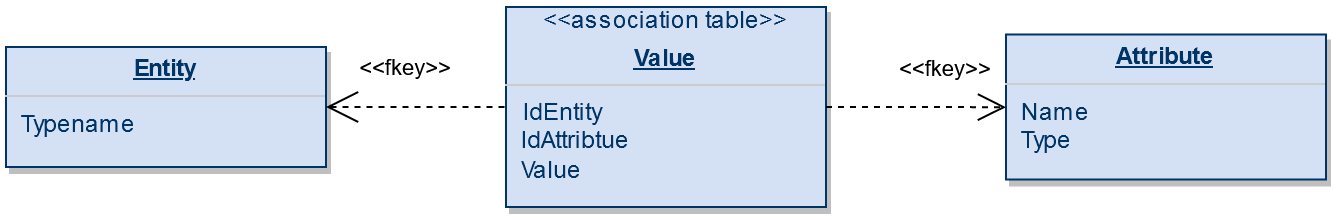
\includegraphics[scale=1.1]{bilder/eavModel.png}
\caption{Datenbankmodell EAV Ansatz}
\end{figure}

Für jeden der drei Teile wird eine Tabelle angelegt. Alle Eigenschaften, die jedes Objekt besitzen soll, bekommen eine Spalte in der Entity Tabelle. Dazu gehört die Id, die in jeder Umsetzung existieren muss, oder auch optionale Werte wie der Zeitpunkt der Erstellung oder der Ersteller des Objekts. Die Definition der dynamischen Attribute, zu der der Name und logische Datentyp gehören, werden in der Attribute Tabelle abgelegt. Die Value Tabelle wird verwendet, um Objekten dynamisch neue Attribute zusammen mit den zugehörigen Werten zuzuweisen. Ein Eintrag in dieser Tabelle benötigt als Fremdschlüssel die Id des Objektss, die Id des Attributs und ein Wert für dieses Attribut. So kann einem Objekt beliebige Attributwerte zugeordnet werden.

Der Einsatz von EAV in einer relationalen Datenbank wird meist als Anti-Pattern bezeichnet oder wird als Indikator für schlechtes Datenbankdesign genommen. Das ist insbesondere der Fall, wenn EAV verwendet wird, um ein höchst generisches Modell zu erstellen, in dem alle Daten abgelegt werden können. Hier spricht man von dem Inner Platform Effekt, wiederum ein Anti-Pattern und Folge von Soft-Coding\cite{JonHeller.2019}. In gewisser weise ist jedoch die Aufgabenstellung, dynamisch Attribute zu Objekten hinzuzufügen und zu entfernen, auch ein Indikator für den Inner Platform Effekt. Daher sollten diese Bedenken ignoriert werden.

Die Probleme bzw. Gefahren durch EAV sind vielfältig\cite{SmithersMike.2013}:
% paragraph*{Data Independence} Noch keine guten Quellen....

%EAV/CR

%Mehrere elemente

\paragraph*{Performance}

Durch die Aufteilung der Informationen einer Entity müssen bei jeder Query mehrere Joins durchgeführt werden. Außerdem ist es nicht möglich, Indizes auf bestimmte Attribute, die Teil besonders vieler Querys sind, zu legen.

\paragraph*{Datenintegrität}

Je nach Komplexität der Umsetzung des \ac{EAV} Models ist die Aufrechterhaltung von Datenintegrität erschwert. In der einfachsten Umsetzung werden alle Attributwerte als Text oder binär abgelegt. Dadurch gehen Tests für logische Werte auf Datenbankebene verloren. Administratoren könnten bei direkter Eingabe von Daten in die Datenbank unlogische Werte eintragen. Außerdem erschwert dieses Vorgehen die Einsicht der gespeicherten Daten. Bei Anwendungsfehlern müssen Support-Mitarbeiter oft basierend auf Anwendungsqualität die Daten auf Datenbankebene auf Fehler untersuchen. Dieses Vorgehen ist durch die Art wie \ac{EAV} Daten ablegt erschwert.

\paragraph*{Aussagen über Datenbestände}

Die Erstellung von Berichten über gespeicherte Daten ist nur mithilfe von speziellen SQL-Befehlen möglich. In normalen relationalen Datenbankschemas sind Aufgabenstellungen wie die Ausgabe aller Einträge einer Tabelle, d.h. einer logischen Struktur, einfacher umsetzbar.

Dennoch wird EAV als möglicher Lösungsweg für verschiedene Probleme vorgeschlagen. Dazu gehören zum einen das Thema dieser Arbeit, dynamische Schemas, aber auch dünn besetzte Daten. Ein großes Einsatzfeld von EAV sind Datenbanken für Daten aus klinischen Studien. Dazu gehören sowohl Open-Source Datenbanken wie Open Source Vista oder kommerzielle Produkte wie ClinTrial oder Clinical. Ein anderes Beispiel ist SenseLab, ein Projekt das Daten zu bestimmten biologischen Objekten im Bereich des Gehirn einmal abspeichert und dazu verschiedene Webmasken anbietet, die je nach Kontext die Daten unterschiedlich präsentieren. Das unterliegende Datenmodell wird in Organization of heterogeneous scientific data using the EAV/CR representation ausführlich beschrieben \cite{Nadkarni.1999}. Es handelt sich um eine Erweiterung des EAV Modells durch Klassen und Relationen.
%Dazu gehören auch die Arbeiten von Piech, der die Performance von EAV mit seinen entwickeltem Modell mit JSON vergleicht.

% Entity Attribute Value Model
% Erklärung inkl. UML
% "Zweckentfremdung" des Schemas -> extrem allgemeines Schema -> MetaDATA
% Gefahr für Performance
% Code-Smell??

\subsection{Speichern von komplexen Daten in LOBs}

Relationale Datenbanken besitzen neben einfachen Datentypen wie \lstinline|int| oder \lstinline|varchar| auch meist einen Typ für komplexe Objekte wie Bilder oder Binärdateien, die nur semi-/ oder nicht strukturiert sind. Dieser Typ wird in der Regel \ac{LOB} genannt. Manche Datenbankanbieter stellen verschiedene Variationen dieses Typs zur Verfügung, etwa Oracles \ac{BLOB}, \ac{CLOB} und \ac{NCLOB} Typen.

Dieser Datentyp kann dazu verwendet werden, Daten mit dynamischen Schema abspeichern. Die binäre Repräsentation des Objekts aus dem Programm direkt abzuspeichern ist nicht empfehlenswert, da sich diese je nach Programmiersprache, Betriebssystem und Programmversion unterscheiden können. Stattdessen werden Austauschformate verwendet. Dafür gibt es zwei oft verwendete Standards: \ac{XML} und \ac{JSON}.

\paragraph*{XML}

XML ist ein Standard des World Wide Web Consortiums für den Austausch von strukturierten Informationen über das Internet. XML Dokumente müssen einer strikten Form von sich öffnenden und schließenden Tags folgen. Diese Tags markieren Elemente, die bestimmte Attribute haben und auch weitere Elemente enthalten können. Mithilfe der Elemente werden die benötigten Informationen des Dokuments abgebildet. \cite{xml.09.10.2018}

Rund um XML haben sich verschiedene Tools entwickelt, die die Arbeit mit dem Format erweitern können. Eines ist XPath, eine Abfragesprache um Informationen aus einem XML Dokument zu extrahieren \cite{xpath.06.04.2021}. Wohlgeformte XML Dokumente, d.h. Dokumente die allen Regeln der XML Definition folgen, bilden eine Baumstruktur. XPath erlaubt es, Knoten basierend auf ihren Namen, Attributen und Position in der Struktur auszuwählen und auszulesen.
Ein weiteres Werkzeug für XML ist XSD, eine Schemabeschreibungssprache für XML Dokumente \cite{xsd.09.10.2018}. XSD ermöglicht es, das Schema bzw. die Struktur von einer Klasse von XML Dokumenten zu definierten. Dafür wird wiederum ein XML Dokument verwendet. Damit lassen sich Dokumente z.B. validieren und ohne Fehler automatisch auslesen.



\paragraph*{JSON}

Laut des offiziellen ECMA-Standards ist:
\begin{quote}
"`JSON (...) a text format that facilitates structured data interchange between all programming languages. JSON 
is syntax of braces, brackets, colons, and commas that is useful in many contexts, profiles, and applications."' \cite[Seite iii]{EcmaInternational.04.02.2021}
\end{quote}

\ac{JSON} basiert auf dem Objektformat von Javascript und ermöglicht es, mit Text Objekte zu beschrieben. Diese Objekte bestehen aus Key-Value Paaren, die als Wert wiederum Objekte, Arrays oder nur einfache Werte haben.
\ac{JSON} wird oft zum Datenaustausch in Webumgebungen verwendet etwa in REST Schnittstellen. Durch das einfache und für den Menschen verständliche Format hat die Popularität von JSON seit der Definition 2006 stetig zugenommen und ersetzt inzwischen XML in manchen Einsatzgebieten.

\begin{figure}
	\begin{adjustbox}{max width=1.4\linewidth,center}
	\centering
	\begin{subfigure}[b]{0.6\textwidth}
		\begin{lstlisting}[language=xml,caption={Beispiel XML}]
	<users>
		<user>
			<firstname>Max</firstname>
			<lastname>Fischer</lastname>
		</user>
		<user>
			<firstname>Lisa</firstname>
			<lastname>Schmidt</lastname>
		</user>
	</users>
\end{lstlisting}
	\caption{per XML}
	\end{subfigure}
	~~~~~~~~
	\begin{subfigure}[b]{0.5\textwidth}
		\begin{lstlisting}[language=json,caption={Beispiel JSON}]
{
	"users" : [
		{ "firstName" : "Max",
		  "lastName"  : "Fischer"
		},
		{ "firstName" : "Lisa",
		  "lastName"  : "Schmidt"
		}
 	]
}
\end{lstlisting}
		\caption{per JSON}
	\end{subfigure}
	\end{adjustbox}
	\caption{Vergleich des Aufbau}
	\label{fig:jsonUML}
\end{figure}

%Vergleich Object JSON xml

Da diese Datenformate generell für viele Einsatzzwecke verwendet werden, bieten Datenbanksysteme oft spezielle Mechanismen um sie in LOBs abzulegen. Entweder durch einen eigenen Datentyp, wie es bei \lstinline|XMLType| für Oracle Database und \lstinline|JSONB| für Postgres der Fall ist, oder Constraints, wie der JSON check in Oracle Database. Dadurch unterscheidet sich die Umsetzung von Datenbank zu Datenbank. Das macht es um so schwieriger, die Features durch eine allgemeine Schnittstelle, wie z.B. \ac{JDBC} in einer Java-Umgebung oder \ac{ODBC}, einzusetzen.

Der Vorteil eines solchen Datentyps ist jedoch, dass dadurch auch Unterstützung durch spezielle Indizes zur Verfügung gestellt werden.

%QUELLE!!!!!!!!!!

% Ablegen Nder dynamischen Teile in Textformatten
% Durch Web nun meist XML oder JSON
% Immer besseres Tooling und Anpassungen da Web und so
% Spezielle Tools für Formateinhaltung
% Inzwischen soger spezieller Datentyp

Datenbankindizes werden dazu verwendet, um Suchanfragen an die Datenbank zu beschleunigen. Ohne einen Index muss die gesamte Tabelle nach passenden Einträgen durchsucht werden. Dieser Vorgang ist als full table scan oder sequentieller Scan bekannt. Dieser Scan ist meistens die letzte Wahl.
Es existieren verschiedene Index Typen, die verschiedene Datenstrukturen und Einsatzzwecke haben.  Am meisten Einsatz finden B-Tree Indizes, die besonders gut geeignet sind, um Einträge mit genauen Werten oder Werten in einem bestimmten Bereich zu finden. Genauer gesagt wird im Index hinterlegt, in welchem Speicherblock mögliche Treffer zu finden sind. 

Die Auswahl von Datenbankensystemen soll basierend auf verfügbare Indizes eingeschränkt werden, da ansonsten keine natürlichen Methoden zur Verbesserung der Performance existieren. Da diese Textformate als spezielle Datentypen abgelegt werden, sollten auch spezielle Indizes verfügbar sein.

Für die Testanwendung wurde JSON verwendet. Diese Entscheidung basiert auf den selben Faktoren, die zur Pri­o­ri­sie­rung von JSON über XML im Bereich der Webentwicklung geführt haben. Dazu gehören in diesem Gebiet die niedrigere Verbosität von JSON, was im selben Zug zu niedrigerem Speicherverbrauch führt, und die höhere Serialisierungsgeschwindigkeit\cite{NurzhanNurseitov.2009}.

Zusätzlich ist zu erwähnen, dass dieser Ansatz die erste Normalform missachtet und dadurch auch keine höheren Normalformen erfüllen kann. Dies wird in Kauf genommen, ähnlich wie die vierte und fünfte Normalform auch oft ignoriert werden. Daher muss mit fehlender Redundanz der Datensätze und den daraus resultierenden Anomalien gerechnet werden. Daher sollte dieser Ansatz mit spezieller Logik erweitert werden, die diese Anomalien verhindern soll.

\subsection{Weitere Lösungsansätze}

Eine weiterer Lösungsweg wäre der sogenannte ``h-store'' von PostgreSQL. h-store beschreibt einen Datentyp, in dem mehrere Key-Value Paare gespeichert werden können. Um diesen Ansatz jedoch komplett umzusetzen müsste zusätzlich ein Weg gefunden werden, den Attributtyp eines Paares abzuspeichern und zu referenzieren. Ein weiteres Problem wären Attribute, die mehrere Werte haben. h-store kann nur einfache Datentypen und keine Listen ablegen. Zu Beginn der Arbeit wurden beide Features als wichtig eingestuft und haben auch das Design des Testprogramms und das JSON Format der serialisierten Objekte beeinflusst. Herausforderungen bei der Umsetzung haben diese Features jedoch in den Hintergrund geschoben. Beide sind in dem Design noch sichtbar, besitzen jedoch keine praktischen Features. Hierzu wird genauer in Kapitel \ref{sec:testaufbau} Testaufbau eingegangen.

%Vllt im Praxisbereich erst durchnehmen?


%#########
%
% NoSQL
%
%#########

\chapter{Moderne Datenbanken}

Seit dem Aufstieg des Internets müssen sich Datenbankentwickler neuen Herausforderungen stellen. Global verfügbare Anwendungen und Dienstleistungen, die von Millionen von Benutzern gleichzeitig verwendet werden, haben andere Anforderungen als die gewohnten tabellarischen Systeme. Dazu gehören größere Datenmengen, komplizierte Beziehungen zwischen Entities, Ausfallresistenz oder dynamische Datenstrukturen. Um diese Herausforderungen zu lösen wurden Abstriche in den gewohnten Stärken von \ac{DBMS}, etwa der Konsistenz der Daten oder das fest definierte relationale Modell, in Kauf genommen. Diese neuen Produkte werden oft unter dem Begriff \ac{NOSQL}-Datenbanken gelistet. Aber auch Datenbanken mit relationalen Modell wurden weiterentwickelt und es entstanden neue Produkte mit neuen Stärken. 

\section{NOSQL}
Ohne Überblick über die verschiedenen Merkmale von \ac{NOSQL}-Datenbanken fällt es schwer, die Aussage zu treffen, ob eine diese Datenbanken zu dem jeweils vorliegendem Anwendungsfall passt. Daher werden in diesem Abschnitt vier Merkmale dieser Datenbanken, basierend auf der Arbeit von Davoudian et al.\cite{Davoudian.2018} vorgestellt, um anschließend zu entscheiden, ob eine dieser Lösungen für unser Problem passt.

\subsection{Datenmodell}

Der prägnanteste Unterschied, der bereits aus der Bezeichnung NOSQL ersichtlich ist, sind die verschiedenen verfügbaren Datenmodelle. Sie ermöglichen es Daten, die nicht in das tabellarische Format passen, abzubilden. Aktuell umfasst der Begriff NOSQL im Groben vier verschiedene bekannte Modelle. Es gibt jedoch auch bereits Produkte, die verschiedene Modelle vereinen oder die den hier genannten nur ähneln.
% möglichkeit, wieter zu unterscheiden

\paragraph*{Key-Value Stores}

Key-Value Stores sind die unrestriktivsten Datenbanken bezüglich ihres Inhalts. Sie legen die Dateien in einem Schlüssel - Wert Format ab. Der Schlüssel, meist ein Merkmal zur Identifikation, ist das einzige Medium zur Interaktion mit der Datenbank und steht für einen Eintrag in der Datenbank. Der Value, der unter einem Key abgelegt wird, kann ein beliebiges Format annehmen. Die Inhalte der Datenbank lassen sich per Schlüssel abfragen, Querys nach bestimmten Werten sind nicht oder nur dank spezieller Features einzelner Datenbanken möglich. Daher finden Key-Value Stores oft in Fällen Einsatz, in denen schnell komplexe Daten abgelegt und abgerufen werden müssen, etwa zur Verwaltung von User-Sessions. Sie lassen sich außerdem weiter unterscheiden nach der Art des Speichermediums. In-Memory Key-Value Stores eignen sich für Caching und ähnliche Anwendungsfälle, in denen die Daten flüchtig sind. Nicht-flüchtige Daten können in persistenten oder hybriden, die sowohl im Arbeitsspeicher als auch auf einer Festplatte agieren, Key-Value Stores abgelegt werden.
Bekannte und beliebte Systeme sind Redis, DynamoDB und Azure Cosmos DB.


\paragraph*{Dokumentendatenbanken}

Dokumentendatenbanken verfolgen denselben Ansatz wie Key-Value Stores, ermöglichen es aber, nur Teile von Werten auszulesen und auch nach bestimmten Werten in Querys zu suchen. Dies geschieht, indem die Werte festgesetzten Formaten folgen. Standardmäßig werden hierfür oft die Formate XML oder JSON verwendet, da diese durch das Web-Umfeld bereits viel Einsatz finden. Relationen zwischen einzelnen Einträge in der Datenbank können mit Fremdschlüsseln abgebildet werden oder direkt ineinander abgelegt werden.

\paragraph*{Wide-Column-Store}

Wide-Column-Stores, auch Column-Family-Stores genannt, ähneln von allen NOSQL Datenmodellen am meisten den der relationalen Datenbanken. Daten werden als Kombination von Reihen und Spalten-Familien, die einer Menge von Spalten entspricht, die in der Regel zusammen aufgerufen werden, dargestellt. Diese Spalten-Familien bilden auch die physische Speichereinheiten.

Beliebte Vertreter dieser Datenbankenart fokussieren sich auf extreme Datenmengen und die Aufteilung dieser Daten auf verschiedene Knoten in einem Cluster. Sowohl Cassandra als auch HBase empfehlen eine Hardwarekonfiguration mit mindestens 3 Knoten.

\paragraph*{Graph-Database}

Graph-Datenbanken legen den Fokus des Daten-Modells auf die Verhältnisse zwischen Entities. Das Ablaufen von Verhältnissen, was in einer SQL Datenbank mit vielen Performance intensiven join-Operationen verbunden wäre, ist eine besondere Stärke dieser Datenbanken. Sie sind in ihrem Datenmodel sehr von der Graphentheorie inspiriert. Dank spezieller Algorithmen können Netzwerkdaten effizient gespeichert werden, wobei es unterschiedliche Verfahren gibt, die jeweils für verschiedene Einsatzzwecke optimiert sind.

Alle NOSQL-Datenmodelle haben ähnliche Anforderungen gegenüber der Modellierung der Informationen. In relationalen Modellen orientiert sich ein Datenbankarchitekt an den Vorgaben der Normalform, um Duplikate in der Datenbank zu vermeiden. Beim Design von NOSQL Schemas liegen die Use-Cases im Vordergrund. Daten werden so abgelegt, das sie performant wieder aufgerufen werden können. Durch die limitierten Abfragewege in NOSQL Datenbanken müssen alle gewünschten Querys abgedeckt werden. Daher ist es manchmal hilfreich, Daten mehrfach in verschiedenen Strukturen abzulegen.
Die Schemafreiheit von manchen NOSQL-Datenbanken bedeutet nicht komplette Freiheit von Datenstrukturen. Damit Daten automatisch von Programmen verarbeitet werden können, muss eine Struktur definiert sein. Dieser Schritt wird in relationalen Datenbanken per SQL erledigt. Datenbankadministratoren beschreiben das Datenbank Schema mithilfe von Datenbank Werkzeugen. NOSQL Datenbanken jedoch verschieben die Verantwortung von der Datenbankebene auf die Anwendungsebene. Die Struktur der Daten wird entweder als richtig impliziert oder muss mithilfe einer bestimmten \ac{DDL} identifiziert und validiert werden. Dadurch wird der Anwendungscode komplexer und unflexibel, eine Eigenschaft, deren Lösung eigentlich DBMS sein sollten. Der Vorteil dieses Vorgehens ist jedoch, dass das Ablegen der Daten, sollten sie beim Abspeichern nicht auf ein Schema getestet werden, schneller erfolgen kann. Der Moment der Validierung wird vom Speicher- zum Lesevorgang verschoben.

\subsection{Datenkonsistenz Modell} \label{ssec:consistency}
Neben dem Datenmodell ist ein weiterer wichtiger Punkt für die Auswahl einer Datenbank die Konsistenz der Daten. Dies ist besonders bei Datenbanken der Fall, die über mehrere Knoten aufgeteilt sind, ein Feature vieler NOSQL Datenbanken. Bei gleichzeitigen Lese- und Schreibvorgängen auf verschiedenen Knoten, die Duplikate der selben Datensätze speichern, muss das Verhalten der Datenbank voraussagbar sein.
Viotti und Vukolic\cite{Viotti.01.12.2015} haben über 50 verschiedene Konsistenz-Modelle untersucht und in Relation zueinander gesetzt. Gröber betrachtet lassen sich diese in verschiedene Kategorien eingliedern.
Der strikteste Konsistenz ist starke Konsistenz, auch als Liniearisierbarkeit bekannt, in der die Reihenfolge der Operationen strikt und fest ist. Am anderen Ende des Spektrums liegt Eventual Consistency, ein Model das den Fokus auf Performance und Verfügbarkeit setzt. Dass Dateneinträge eventuell veraltet sein können, wird ignoriert und man erwartet nur, dass irgendwann am Schluss alle Einträge konsistent sind.

\subsection{Partitionierung}
Partitionierung beschreibt die Möglichkeit, Daten auf mehrere Knoten aufzuteilen. Dies geschieht meist auf horizontaler Ebene, d.h. Aufteilung der Daten auf mehrere Maschinen. Dies ermöglicht schnelleren Zugriff basierend auf geographischen Faktoren, als auch parallelen Zugriff auf unterschiedliche Datensätze. Dieser Vorgang, auch als Sharding bekannt, ist mit den meisten relationalen Datenbanken nicht möglich. Man kann Datenbanken basierend auf verschiedenen Partitionierungsfokusse unterscheiden, etwa zur Verteilung der Daten um die Auslastung von Maschinen auszugleichen oder um eine Mindestanzahl an Backups versichern zu können.

\subsection{CAP Theorem}

Das CAP Theorem beschreibt das Verhältnis von Konsistenz, Verfügbarkeit und Aufteilungstoleranz.
\begin{itemize}
\item Consistency (C) - 
Die Konsistenz der Daten, vgl. \ref{ssec:consistency}
\item Availability (A) - 
Die Verfügbarkeit und Reaktionsgeschwindigkeit des Systems, um sowohl Lese- als auch Schreibanweisungen durchzuführen
\item Partition Tolerance (P) - 
Die Toleranz, die das System gegenüber Teilausfällen, z.B. einzelner Nodes, zeigt.

\end{itemize}

Das Theorem besagt: 
 
\begin{quote}
"`You can have at most two of these properties for any shared-data system"' \cite[Folie 14]{Brewer.2000}
\end{quote}

So lassen sich verteilte Datensysteme als CA, CP oder AP einstufen. Traditionelle relationale Single Node Datenbanken zum Beispiel fallen unter CA, d.h. nur konsistent und verfügbar, da ein Ausfall eines Knotens das gesamte System stilllegt. Genau betrachtet wäre das jedoch keine Spaltung sondern ein Komplettausfall. Systeme, die eine gewisse Toleranz gegenüber Spaltung erreichen wollen, müssen Abstriche in einem der beiden anderen Themen in Kauf nehmen. Dies basiert auf der Verteiltheit der Daten. Um die aktuellste Version eines Datensatzes zu bekommen, müssen alle zuständigen Nodes abgefragt werden. Dies erhöht jedoch die Laufzeit von Anfragen. Ein Administrator muss also basierend auf dem Anwendungsfall die Wahl zwischen Datenbanksystemen bzw. Datenbank-Konfigurationen treffen.

Das Theorem, die wissenschaftliche Untersuchung des Theorems und der Umgang damit wird jedoch auch kritisiert. Viele Datenbanken erfüllen nicht die strengen Anforderungen des Beweises des Theorems, identifizieren sich jedoch trotzdem als eine der Variationen. Es kann auch sein, dass Datenbanken diesen Anforderungen nur entsprechen, falls sie in einem bestimmten Modus laufen. \cite{MartinKleppmann.2015}

Es lohnt sich dennoch es zu betrachten, da es hilft, grundlegende Unterschiede von verteilten Datenbanksystemen zu erkennen. 



Die beschriebenen Eigenschaften von NOSQL Datenbanken geben Einblick über ihre Fokusse. Diese liegen hauptsächlich auf verteilten Datenbanken, mit eingeschränkter Konsistenz der Daten und maximaler Anzahl von Querys. 
Sie eignen sich für extreme Datenmengen und Daten mit speziellen Format. Diese Daten können meist nur in einer bestimmten Form abgerufen werden, da nur in bestimmten Datenmodellen Ad-Hoc Querys unterstützt werden. Um das zu umgehen, werden oft die selben Daten mehrfach abgespeichert, was den Grundgedanken der Normalisierung des Modells in traditionellen Datenbanken ignoriert.
Weitere ignorierte Faktoren, die durch die Spezialisierung auf besondere Aufgabenstellungen entsteht und Administratoren von traditionellen Datenbanken am Herzen liegen, sind u.A. der Einhaltung des \ac{ACID} Modells und der Verlust von bekannten und verinnerlichten Tools. Das macht es oft schwer, NOSQL Datenbanken neu in bereits etablierten Umgebungen einzuführen, insbesondere da die Änderung von Maxime stets mit Skepsis verbunden ist.

Im Idealfall werden NOSQL Datenbanken parallel mit relationalen Datenbanken verwendet, wobei auch dieses Vorgehen durch Konsistenz und Ausfalls-Verhalten eingeschränkt und erschwert wird. Und mit Steigerung der Komplexität der gesamten Architektur von Anwendungen steigt auch die Möglichkeit von Fehlern. Da \ac{OLTP} Anwendungen, besonders wenn Rechnungs- oder Bankdaten bearbeitet werden, meist auf relationalen Datenbanken und ihren Stärken basieren, konzentriert sich diese Arbeit in der praktischen Analyse auf Methoden zur Implementierung des dynamischen Datenmodells in relationalen Datenbanken. Mit genügend Planung und wenn der Verwendungszweck nicht perfekte Konsistenz erlaubt, würden sich insbesondere Wide-Column- und Key-Value-Stores auch für die Aufgabenstellung qualifizieren.

% Key-value
%  

% Immer dieses Web + BigData -> Krass voll schwer!!!

% 4? Punkte für NOSQL

% - Datamodel (größer Ausführen)

%(kleiner behandeln)
%- Linearilisierbarkeit / Consistency 
%- Partitionierung
%- CAP Principle

%=> für uns interessant: column family store, document store => ABER: weder sql noch transactionen => Nur als Vergleich betrachten (neu = besser?)

% Vermeidung von pro-innovation bias

\section{NewSQL}

Ein weiterer Begriff, der sich in den 2010er Jahren etablierte, ist NewSQL. Unter diesem Schlagwort werden alle Datenbanken eingegliedert, die Lehren aus den neuen Technologien der NOSQL Datenbanken ziehen, selbst aber wie relationale Datenbanken agieren. Da NOSQL für Not Only SQL steht, ist NewSQL eine Unterkategorie von NOSQL. 
Stonebraker \cite{MichaelStonebraker.2011} identifiziert zwei Anwendungsgebiete von New SQL. Zum einen Anwendungen, die extreme Datenmengen verarbeiten müssen, aber nicht auf Features wie SQL als Abfragesprache und die ACID Eigenschaften von Transaktionen verzichten wollen. Dazu gehören typische BigData Szenarien wie z.B. Webanwendungen mit extrem vielen Benutzern und Transaktionen pro Minute.
 
Der andere Fall sind Anwendungen, die sowohl analytische als auch transaktionale Use-Cases unterstützen sollen. Systeme dieser Art, die \ac{OLTP} und \ac{OLAP} verbinden, werden auch \ac{HTAP} genannt. Sie ermöglichen die Echtzeitanalyse von Geschäftsdaten. Diese Anforderung lässt sich auf verschiedenen Wegen implementieren. Giceva und Sadoghi \cite{Giceva.2018} identifizierten zwei Kernpunkte, in denen sich HTAP Systeme unterscheiden können. Als erstes bei Datenrepräsentation, d.h. der Einsatz von entweder Row- oder Columnstores oder eine Kombination der beiden. Und zum anderen bei Daten Replikation, insbesondere ob nur eine oder mehrere Kopien der Daten im physikalischen Speicher vorliegt.

Diese beiden Szenarien treffen jedoch nicht genau unsere Problemstellung. Trotzdem gäbe es interessante Kandidaten. Insbesondere In-Memory Stores, d.h. Datenbanken, die einen Teil der Daten in flüchtigen und dadurch in besonders schnellen Speicher hält, könnten den der benötigten Unterschied für eine akzeptable  Performance ausmachen. Diese Datenbanken haben dadurch jedoch auch größere Anforderungen an die benötigte Hardware, besonders bei der Menge an Arbeitsspeicher. 
Da die verfügbare Testmaschine nicht diese Anforderungen erfüllen konnte, wurden In-Memory Datenbanken nicht weiter in Erwägung gezogen.

%Außerdem:

%- In Memory DBs
%- Column based Storage
%- Apache Drill


 